%%%%%%%%%%%%%%%%%%%%%%%%%%%%%%%%%%%%%%%%%
% Beamer Presentation
% LaTeX Template
% Version 1.0 (10/11/12)
%
% This template has been downloaded from:
% http://www.LaTeXTemplates.com
%
% License:
% CC BY-NC-SA 3.0 (http://creativecommons.org/licenses/by-nc-sa/3.0/)
%
%%%%%%%%%%%%%%%%%%%%%%%%%%%%%%%%%%%%%%%%%

%----------------------------------------------------------------------------------------
%	PACKAGES AND THEMES
%----------------------------------------------------------------------------------------

\documentclass{beamer}

\mode<presentation> {

% The Beamer class comes with a number of default slide themes
% which change the colors and layouts of slides. Below this is a list
% of all the themes, uncomment each in turn to see what they look like.

%\usetheme{default}
%\usetheme{AnnArbor}
%\usetheme{Antibes}
%\usetheme{Bergen}
%\usetheme{Berkeley}
%\usetheme{Berlin}
%\usetheme{Boadilla}
%\usetheme{CambridgeUS}
%\usetheme{Copenhagen}
%\usetheme{Darmstadt}
%\usetheme{Dresden}
%\usetheme{Frankfurt}
%\usetheme{Goettingen}
%\usetheme{Hannover}
%\usetheme{Ilmenau}
%\usetheme{JuanLesPins}
%\usetheme{Luebeck}
\usetheme{Madrid}
%\usetheme{Malmoe}
%\usetheme{Marburg}
%\usetheme{Montpellier}
%\usetheme{PaloAlto}
%\usetheme{Pittsburgh}
%\usetheme{Rochester}
%\usetheme{Singapore}
%\usetheme{Szeged}
%\usetheme{Warsaw}

% As well as themes, the Beamer class has a number of color themes
% for any slide theme. Uncomment each of these in turn to see how it
% changes the colors of your current slide theme.

%\usecolortheme{albatross}
%\usecolortheme{beaver}
%\usecolortheme{beetle}
%\usecolortheme{crane}
%\usecolortheme{dolphin}
%\usecolortheme{dove}
%\usecolortheme{fly}
%\usecolortheme{lily}
%\usecolortheme{orchid}
%\usecolortheme{rose}
%\usecolortheme{seagull}
%\usecolortheme{seahorse}
%\usecolortheme{whale}
%\usecolortheme{wolverine}

%\setbeamertemplate{footline} % To remove the footer line in all slides uncomment this line
%\setbeamertemplate{footline}[page number] % To replace the footer line in all slides with a simple slide count uncomment this line

%\setbeamertemplate{navigation symbols}{} % To remove the navigation symbols from the bottom of all slides uncomment this line
}
\usepackage[latin1]{inputenc}

\usepackage{graphicx} % Allows including images
\usepackage{booktabs} % Allows the use of \toprule, \midrule and \bottomrule in tables
%\usepackage{bibtex}

%\usepackage{enumitem}
%\newcounter{enumit}
\newcounter{cste}

\definecolor{azure}{rgb}{0.0, 0.5, 1.0}

%\bibliographystyle{chicago}

%\usepackage{enumitem}
%\newlist{arrowlist}{itemize}{1}
%\setlist[arrowlist]{label=$\Rightarrow$}

\setbeamertemplate{enumerate items}[ball]

%----------------------------------------------------------------------------------------
%	TITLE PAGE
%----------------------------------------------------------------------------------------

\title[word embeddings]{Drawing a "map of words": word embeddings and applications to machine translation and sentiment analysis} % The short title appears at the bottom of every slide, the full title is only on the title page

\author{Mostapha Benhenda} % Your name
\institute[] % Your institution as it will appear on the bottom of every slide, may be shorthand to save space
{
Artificial Intelligence Club, Kyiv \\ % Your institution for the title page
\medskip
\textit{mostaphabenhenda@gmail.com} % Your email address
}
\date{\today} % Date, can be changed to a custom date

\begin{document}

\begin{frame}
\titlepage % Print the title page as the first slide
\end{frame}

\begin{frame}
\frametitle{Overview} % Table of contents slide, comment this block out to remove it
\tableofcontents % Throughout your presentation, if you choose to use \section{} and \subsection{} commands, these will automatically be printed on this slide as an overview of your presentation
\end{frame}

%----------------------------------------------------------------------------------------
%	PRESENTATION SLIDES
%----------------------------------------------------------------------------------------

%------------------------------------------------
\section{Introduction} % Sections can be created in order to organize your presentation into discrete blocks, all sections and subsections are automatically printed in the table of contents as an overview of the talk
%------------------------------------------------

%\subsection{Subsection Example} % A subsection can be created just before a set of slides with a common theme to further break down your presentation into chunks

\begin{frame}
\frametitle{Introduction}

We want to compute a "map of words", i.e. a representation: 

\[ R: \mbox{Words}= \{ w_1,...,w_N \} \rightarrow  \mbox{Vectors} = \{ R(w_1),..., R(w_N) \} \subset \mathbb{R}^d \]
 
 such that:
 
\begin{align*}
   w_i  &\approx w_j & \text{(meaning of words)}
\end{align*} 
 
is equivalent to:

\begin{align*}
  R( w_i)  &\approx R(w_j) & \text{(distance of vectors)}
\end{align*} 
 


\end{frame}


\begin{frame}
These vectors are interesting because:

\begin{itemize}
\item the computer can "grasp" the meaning of words, just by looking at the distance between vectors.
\item We can feed prediction algorithms (linear regression,...) with these vectors, and hopefully get good accuracy, because the representation is "faithful" to the meaning of words.
\end{itemize}

\end{frame}



\begin{frame}

For example, if we have the list of words: 

\bigskip

\begin{center}
cat, dog, mouse, house

\end{center}

\bigskip

We expect the most distant word to be: ?



\end{frame}

\begin{frame}



\begin{figure}
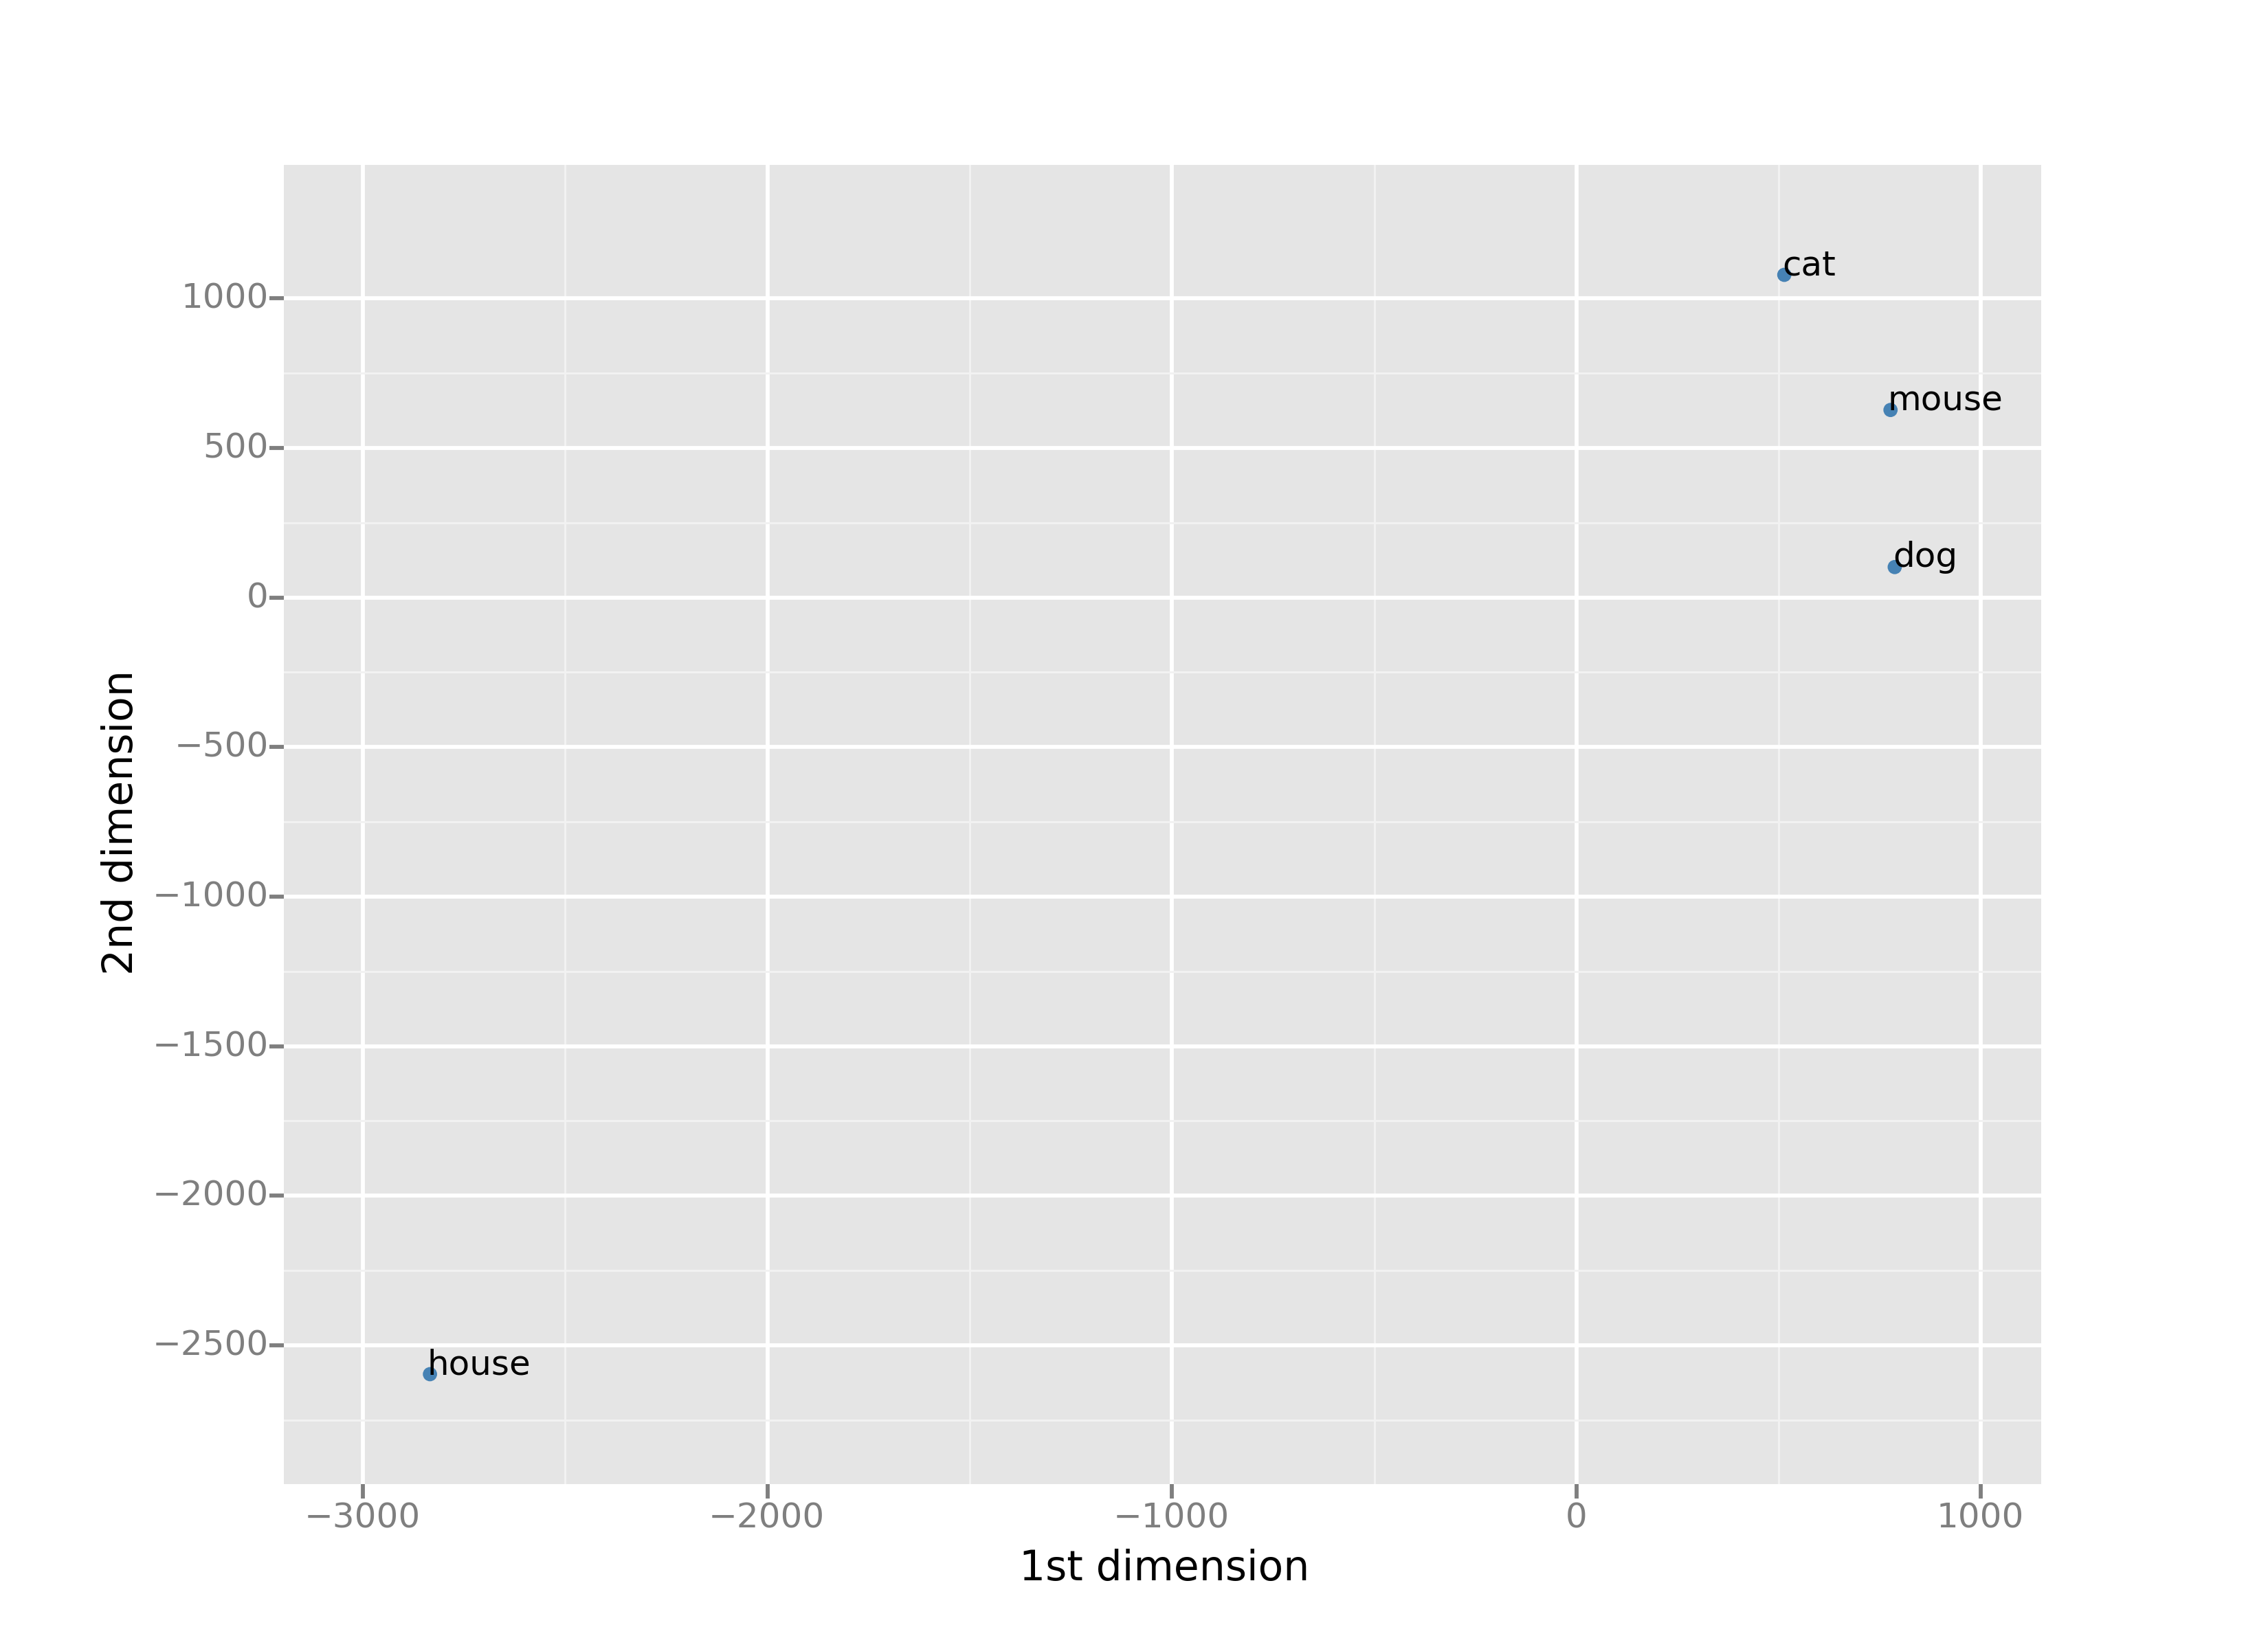
\includegraphics[width=0.85\linewidth]{wordsinenglishtsnesklearn.png}
\end{figure}


(this is a 2-dimensional visualization of a 300-dimensional space, using t-SNE, a visualization technique that preserves clusters of points)


\end{frame}



\begin{frame}
Even better, we can sometimes make additions and substractions of vectors, and draw parallelisms. For example, 

\bigskip

\begin{center}
king + woman - man $\approx$ ?
\end{center}

\end{frame}



\begin{frame}



\begin{figure}
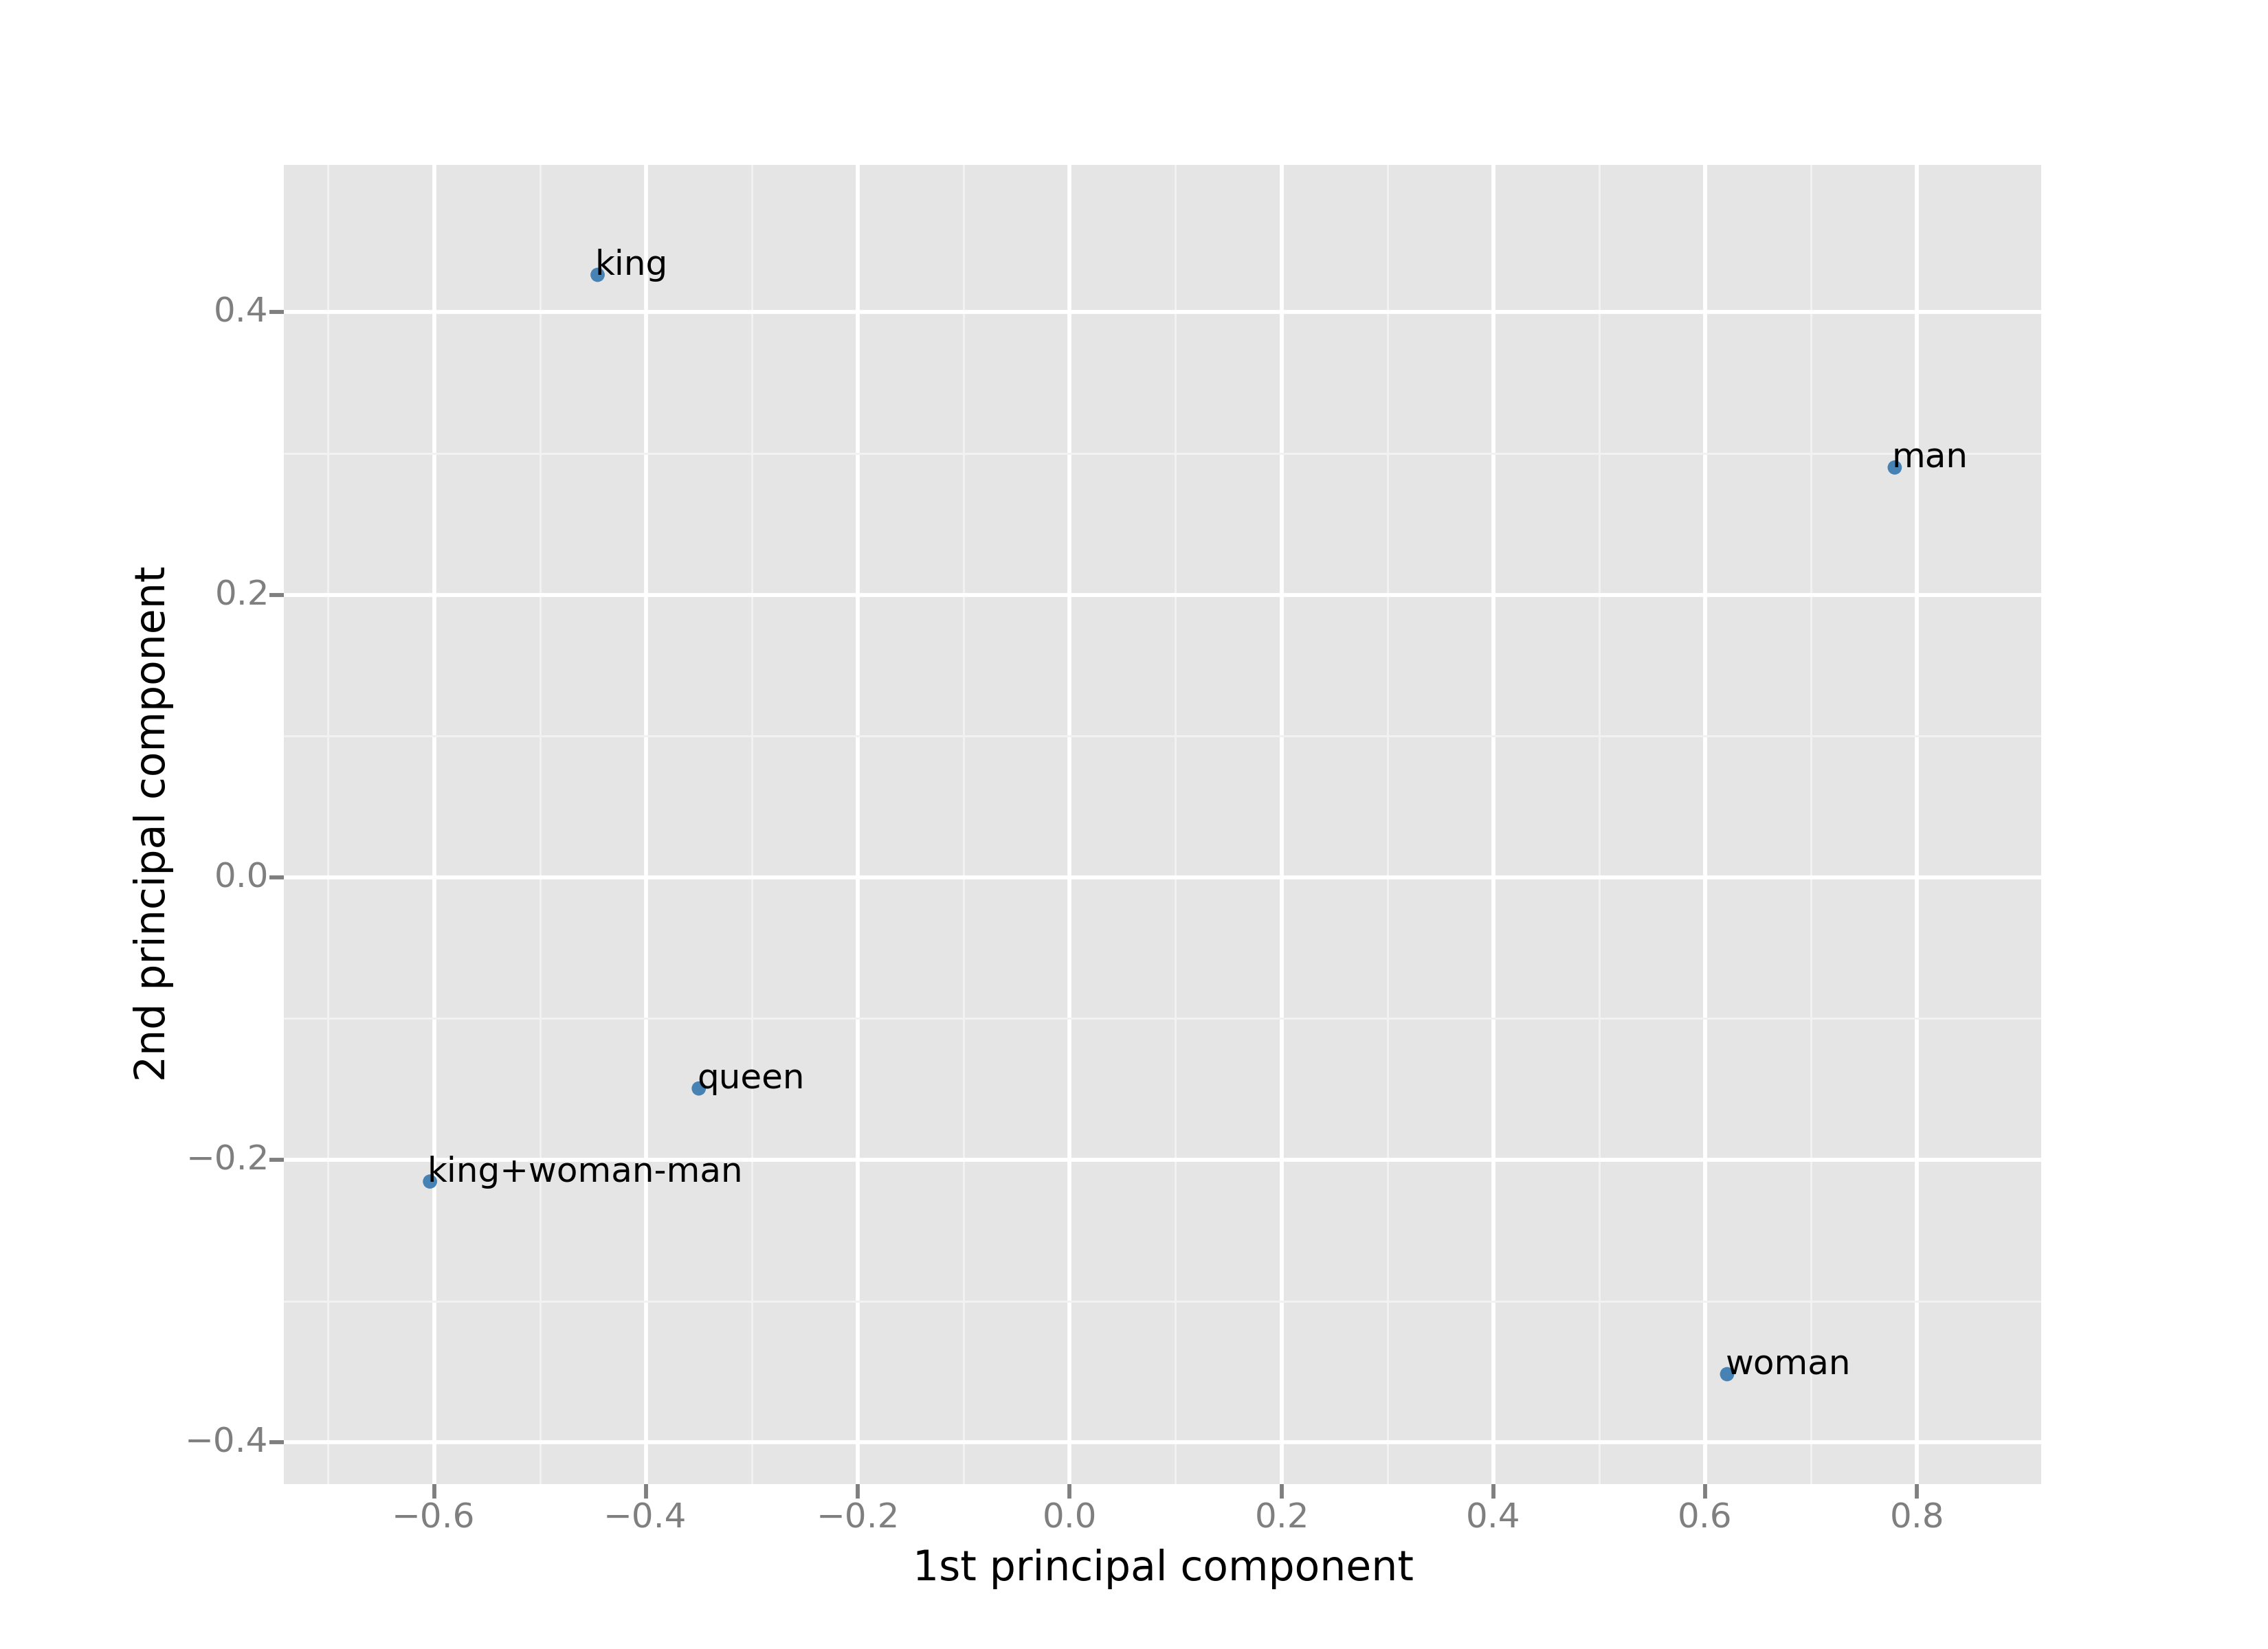
\includegraphics[width=0.85\linewidth]{wordsinenglishanalogyplus.png}
\end{figure}


(2-dimensional visualization of a 300-dimensional space, using PCA, a visualization technique that preserves parallelisms)


\end{frame}
	

\begin{frame}
\begin{itemize}
\item Idea behind all algorithms (Word2vec, GloVe,...): "You shall know a word by the company it keeps" (John R. Firth, 1957)
\item The more often 2 words are near each other in a text (the training data), the closer their vectors will be.
\item We hope that 2 words have close meanings if, statistically, they are often near each other.
\end{itemize}

So we need quite big datasets:


\begin{itemize}
\item Google News English: 100 Billion words
\item Wikipedia French or Spanish: $\simeq$ 100 Million words
\item MT 11 French: 200 Million words
\item MT 11 Spanish: 84 Million words 


\end{itemize}

\end{frame}
	
\begin{frame}

\section{Applications}	

\frametitle{Application to machine translation}	
	
\subsection{Machine translation}	






Idea: we compute maps of all English words, all French words, and we "superpose" the 2 maps, and we should get an English/French translator.



\begin{figure}
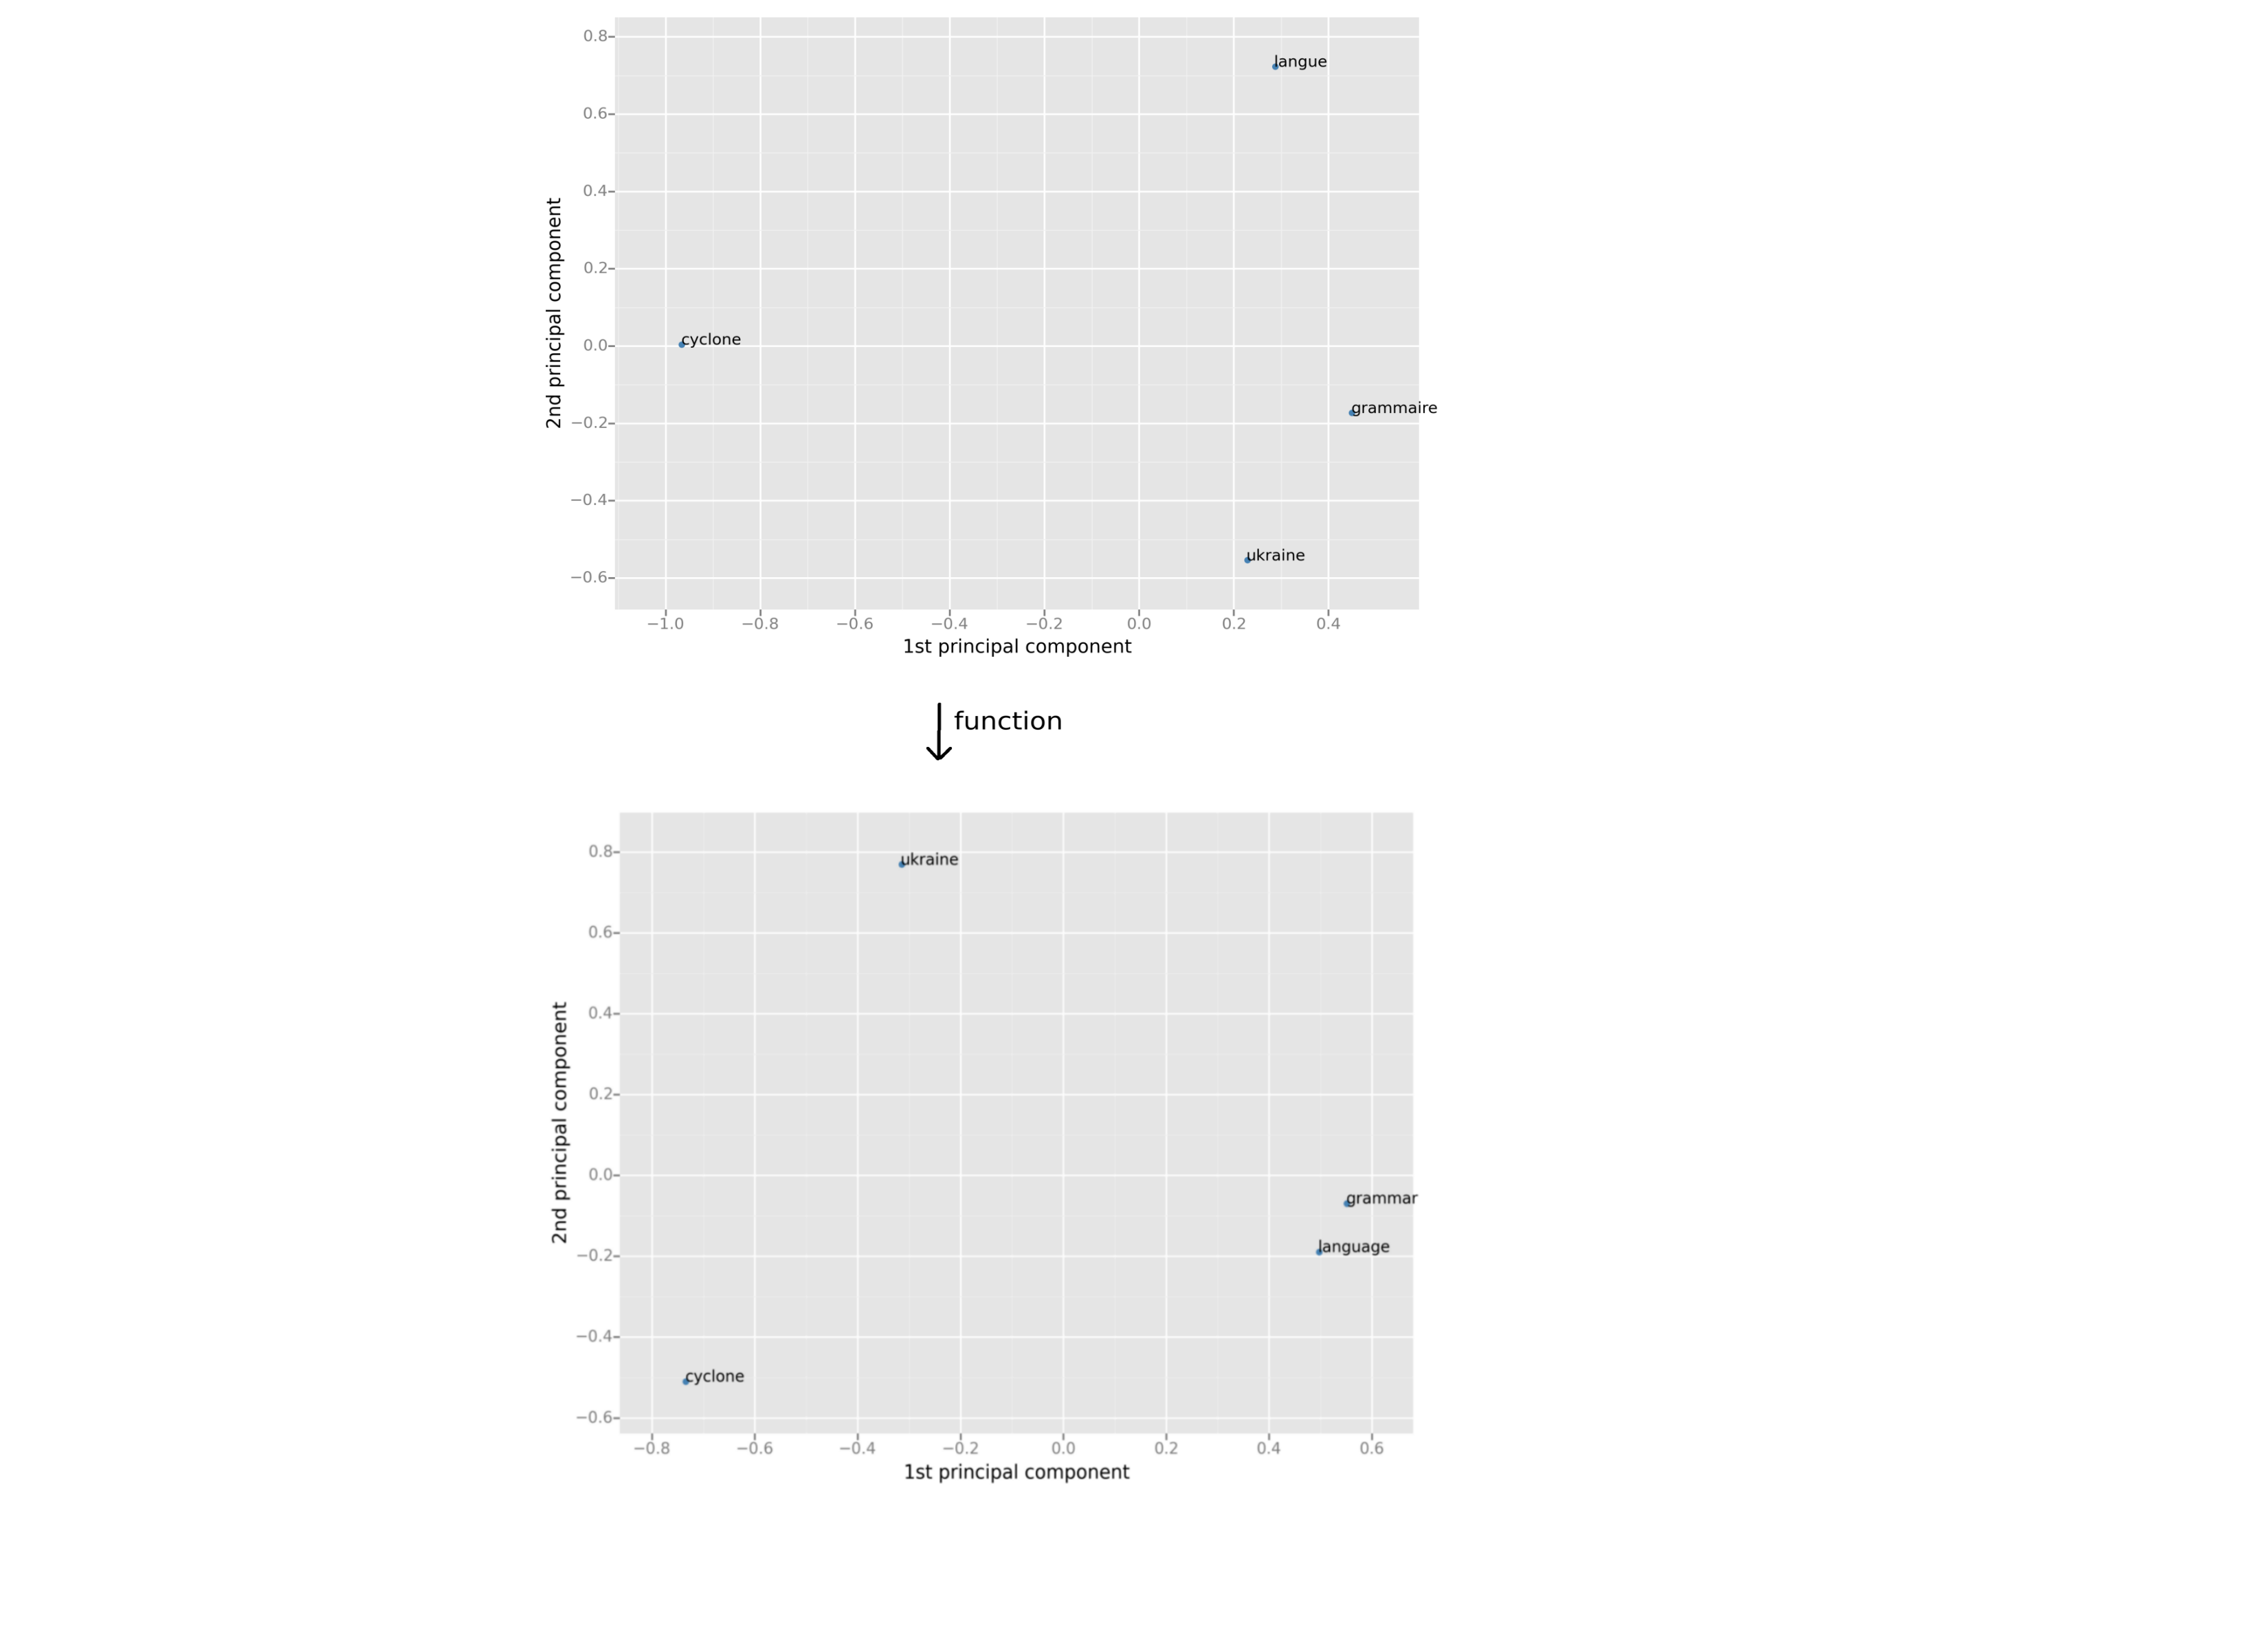
\includegraphics[width=0.85\linewidth]{functionfrenchenglish.png}
\end{figure}


%\end{arrowlist}

%Concretely, we train a function: $\{ \mbox{English vectors} \} \rightarrow \{ \mbox{French vectors} \}$ that minimizes quadratic error.
\end{frame}	


\begin{frame}
\begin{itemize}
\item \cite{mikolov132} (from Google), made an English $\rightarrow$ Spanish translator (among other languages). 

\item I tried to reproduce their results for French $\rightarrow$ English, 

and French $\rightarrow$ Spanish.

\item Using their algorithm Word2vec, they trained their vectors on the dataset MT 11, and on Google News.

\item I did the same on MT 11 and Wikipedias for French and Spanish (trained with Gensim package in Python), and I used their Google News-trained vectors for English.

\end{itemize} 
 
\end{frame}

\begin{frame}

\begin{itemize}

\item Then they took the list of the 5000 most frequent English words, and their Google translation in Spanish.

\item They train a linear transformation $W$ that approximates the English $\rightarrow$ Spanish translation, i.e. they take $W$ that minimizes:

\[  \sum_{i=1}^{5000} \| W(v_i) - G(v_i)  \|^2 \]

where $G(v_i)$ is the Google-translation of $v_i$.


\end{itemize}

\end{frame}

\begin{frame}


\begin{itemize}



\item They test the accuracy of $W$ on the next 1000 most common words of the list (1-accuracy). They also test the accuracy up to 5 attempts, i.e. they test if $G(v_i)$ belongs to the 5 nearest neighbors of $W(v_i)$ (5-accuracy). 

\item I did (almost) the same for French $\rightarrow$ English, and French $\rightarrow$ Spanish. 

\bigskip

\item code available here: https://drive.google.com/

open?id=0B86WKpvkt66BY09TSHJoekRqZjg\&authuser=0  

\item computer-intensive task, I recommend using Amazon Web Services, or similar. 

\end{itemize}

\end{frame}

\begin{frame}

\frametitle{Results}

\begin{itemize}
\item Mikolov, English $\rightarrow$ Spanish: 
\begin{table}
\begin{tabular}{l l l}
\toprule
\textbf{Training data} & \textbf{1-accuracy} & \textbf{5-accuracy}\\
\midrule
Google News & 50\% & 75\% \\
MT 11 & 33\% & 51\% \\
\bottomrule
\end{tabular}
%\caption{Table caption}
\end{table}


\item Me, French $\rightarrow$ Spanish: 
\begin{table}
\begin{tabular}{l l l}
\toprule
\textbf{Training data} & \textbf{1-accuracy} & \textbf{5-accuracy}\\
\midrule
Wikipedia & na & $<$10\% \\
MT 11 & 25\% & 37\% \\
\bottomrule
\end{tabular}
%\caption{Table caption}
\end{table}

\pause

French (Wikipedia) $\rightarrow$ English (Google News) 10-accuracy: $<10\%$.




\end{itemize}

\pause 

My conclusion: Wikipedia = cauchemar !



\end{frame}


\begin{frame}
\subsection{Sentiment analysis of movie reviews}

\frametitle{Sentiment analysis of movie reviews}

\begin{itemize}
\item Goal: we want to determine if a movie review is positive or negative. 
\item Toy problem in machine learning: reviews are ambiguous, emotional, full of sarcasm,... 
\item Long-term goal: computer can understand emotions. 
\item Commercial applications of sentiment analysis: 
\begin{itemize}
\item marketing: customer satisfaction,... 
\item finance: predict market trends,...
\end{itemize} 
 
\item Example of review: "This movie contains everything you'd expect, but nothing more". 

\end{itemize}

\end{frame}

\begin{frame}

\subsubsection{ Vector averaging (Kaggle tutorial)}

\frametitle{Vector averaging (Kaggle tutorial)}

We work on the IMDB dataset. To predict the sentiment (+ or -) of a review:

\begin{itemize}
\item let the vector of a review be the average of the vectors of its words
\item We use these vectors as input to a supervised learning algorithm (e.g. SVM, random forests...)
\item We get $83\%$ accuracy (not the best method on this Kaggle challenge, easier methods work better)

\item Limitation of the method: the order of words is lost, because addition is a commutative operation. 
\end{itemize}

\end{frame}

\begin{frame}



\subsubsection{Convolutional Neural Networks (deep learning)}

\frametitle{Convolutional Neural Networks (deep learning) (work in progress)}

\begin{itemize}
\item CNN are biology-inspired neural network models, initially introduced for image processing.
\item they preserve spatial structure: the input is a $n \times m$ matrix (the pixels of the image)
\item but here, the input is a sentence (with its "spatial structure" preserved): 
\end{itemize}

\begin{figure}
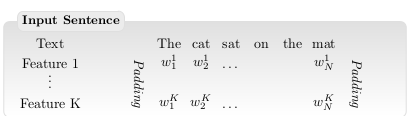
\includegraphics[width=1.0\linewidth]{collobert.png}
\caption{source: \cite{collobert11}}
\end{figure}


\end{frame}

\begin{frame}

\subsection{Other applications of word embeddings}

\frametitle{Other applications of word embeddings}

\begin{itemize}
\item Innovative search engine (ThisPlusThat), where we can subtract queries, for example:

\begin{center}
pizza + Japan -Italy $\rightarrow$ sushi
\end{center}  
 
\item Recommendation systems for online shops
\end{itemize}


\end{frame}

\begin{frame}

\section{Example of word embedding algorithm: GloVe}

\frametitle{Example of word embedding algorithm: GloVe}

GloVe: "Global Vectors" algorithm made in Stanford by \cite{pennington14}. There are 2 steps:

\begin{enumerate}
\item Build the co-occurrence matrix $X$ from the training text
\item Factorize the matrix $X$ to get vectors
\end{enumerate}


\bigskip

\subsection{Build the co-occurrence matrix $X$}

\textbf{1. Build the co-occurrence matrix $X$:} 

For the first step, we apply the principle "you shall know a word by the company it keeps": 

\end{frame}

\begin{frame}

\begin{itemize}
\item The \colorbox{yellow}{\textit{context window}} $C(w)$ of size $2$ of the word $w$= \colorbox{azure}{Ukraine}  (for example), is given by: 
\end{itemize}

\begin{center}
The national \colorbox{yellow}{flag of} \colorbox{azure}{Ukraine} \colorbox{yellow}{is yellow} and blue.
\end{center}

(in practice, we take the context window size around 10)


\bigskip

\begin{itemize}
\item The number of times 2 words $i$ and $j$ lie in the same context window is denoted by $X_{i,j}$. 
\item The symmetric matrix $X=(X_{i,j})_{1 \leq i,j \leq N}$ is the \textit{co-occurrence matrix}.

\end{itemize}

\end{frame}

\begin{frame}


\subsection{Matrix factorization}

\textbf{2. Factorize the co-occurrence matrix $X$:}


\begin{itemize}
\item To extract vectors from a symmetric matrix, we can write:

\[   X_{i,j} = \, <v_i,v_j>   \; \; \; \; v_i \in \mathbb{R}^d, \]
 
where $d$ is an integer fixed by us a priori (a hyperparameter). i.e. we can write:

\[   X = \mbox{Gram}(v_1,...,v_N)    \]

\item This formula does not give a good empirical performance, but:

for any scalar function $f$, $(f(X_{i,j}))_{1 \leq i,j \leq N}$ is still a symmetric matrix. 

\item Let's find $f$ that works!
\end{itemize}

\end{frame}

\begin{frame}

\begin{itemize}
\item Let $i$, $j$ be 2 words, for example: $i$= fruit, $j$=house. The third word $k$=apple has a meaning closer to fruit than to house, so $X_{i,k}/X_{j,k}$ is small.  
\item If $k$=room (closer to "house" than to "apple"), then $X_{i,k}/X_{j,k}$ is large.
\item If $k$= sky (far from both "house" and "apple"), then $X_{i,k}/X_{j,k} \simeq 1$.
\end{itemize} 

$\rightarrow$ the ratio of co-occurrences $X_{i,k}/X_{j,k}$ is important to capture meaning of words. So we should look at $f( X_{i,k}/X_{j,k})$.

\begin{itemize}
\item On the other hand, if we want to combine 3 vectors and the scalar product in a "natural" way, we do not have much choice:

\pause

\[  <v_i-v_j,v_k>=f(X_{i,k}/X_{j,k})    \]

\pause 

\item We also have:
\[  <v_i,v_k> - <v_j,v_k> = f(X_{i,k})- f(X_{j,k})    \]


\item So $  f= \log$
\end{itemize}

\end{frame}

\begin{frame}
\begin{itemize}
\item We cannot factorize the matrix $\log X$ explicitly, i.e. we cannot directly compute $v_i,v_j$ such that:

\[ <v_i,v_j> = \log X_{i,j} \]


\item but we compute an approximation, by minimizing a cost function $J$:

\[  \min_{v_1,...,v_N}  J(v_1,...,v_N) \sim  \sum_{i,j=1}^N  \left( <v_i,v_j> - \log X_{i,j}    \right)^2   \]

\item To do that, we use gradient descent (standard method).
  
\end{itemize}
\end{frame}

\begin{frame}
Looks like cooking, but:
\begin{itemize}
\item good empirical performance (at least similar to Word2vec)
\item cost function $J$ similar to Word2vec
\item GloVe model is analogous to Latent Semantic Analysis (LSA). In LSA:
\begin{itemize}
\item co-occurrence matrix is a word-document matrix X (In GloVe: word-word matrix)
\item we factorize $\sim \log (1+X_{i,j}) $ (SVD, not Gram matrix)
\end{itemize}

\end{itemize}

\bigskip

Conclusion: GloVe model is worth to study!

\end{frame}



\section{Future work}

\begin{frame}

\frametitle{Future work} 


\begin{itemize}
\item Doc2vec \cite{mikolov14}  
\item Deep learning (Convolutional Neural Networks): Natural Language Processing (almost) from Scratch \cite{collobert11}

\pause

\item Suggestion: have a deep learning study group in Kyiv!
\item Applications of deep learning: NLP, images, videos, speech,...

$\rightarrow$ money!!
\end{itemize}

\pause

Pre-requisites: a little of:

\begin{enumerate}
\item coding (Python or Matlab or Java...)
\item linear algebra (matrix multiplication)
\item calculus (chain rule)
\item enthusiasm!
\end{enumerate}

\begin{center}
Register at: http://deeplearningkyiv.doorkeeper.jp/
\end{center}

\end{frame}
%------------------------------------------------

%------------------------------------------------

\begin{frame}
\section{References}

\frametitle{References}
\footnotesize{
\begin{thebibliography}{99}


\bibitem[Bergstra et al. 2010]{theano} Bergstra, J., Breuleux, O., Bastien, F., Lamblin, P., Pascanu, R., Desjardins, G., ... \& Bengio, Y. (2010)
\newblock Theano: a CPU and GPU math expression compiler
\newblock \emph{Proceedings of the Python for scientific computing conference (SciPy)}, (Vol. 4, p. 3) 




\bibitem[Collobert et al. 2011]{collobert11} Collobert, R., Weston, J., Bottou, L., Karlen, M., Kavukcuoglu, K., \& Kuksa, P. (2011)
\newblock Natural language processing (almost) from scratch
\newblock \emph{The Journal of Machine Learning Research}, 12, 2493-2537 


\bibitem[Mikolov et al. 2013]{mikolov131} Mikolov, T., Sutskever, I., Chen, K., Corrado, G. S., \& Dean, J. (2013)
\newblock Distributed representations of words and phrases and their compositionality
\newblock \emph{Advances in Neural Information Processing Systems} pp. 3111-3119

\bibitem[Mikolov et al. 2013]{mikolov132} Mikolov, T., Quoc V. Le, Sutskever, I. (2013)
\newblock Exploiting similarities among languages for machine translation
\newblock \emph{arXiv preprint arXiv:1309.4168.} 



\end{thebibliography}
}
\end{frame}

\begin{frame}
\frametitle{References}
\footnotesize{
\begin{thebibliography}{99}

\bibitem[Mikolov et al. 2014]{mikolov14} Mikolov, T., Quoc V. Le (2014)
\newblock Distributed representations of sentences and documents
\newblock \emph{arXiv preprint arXiv:1405.4053.} 


\bibitem[Pennington, Socher, Manning, 2014]{pennington14} Pennington, J., Socher, R., \& Manning, C. D. (2014)
\newblock Glove: Global vectors for word representation
\newblock \emph{Proceedings of the Empiricial Methods in Natural Language Processing (EMNLP 2014)}, 12.


\bibitem[{\v R}eh{\r u}{\v r}ek and Sojka, 2010]{rehurek10} {\v R}eh{\r u}{\v r}ek, R., \& Sojka, P. (2010)
\newblock Software framework for topic modelling with large corpora
\newblock \emph{Proceedings of the Empiricial Methods in Natural Language Processing (EMNLP 2014)}, 12.


\end{thebibliography}
}
\end{frame}

%------------------------------------------------

%----------------------------------------------------------------------------------------

\end{document} 